% !TEX root = ../main.tex
\chapter{Experiments}
\label{ch:experiments}

In this chapter, the objective is to address the research questions of this study through a series of experiments. The experiments performed in this study involve solving the "Lunar Lander" and "Bipedal Walker" control tasks from the OpenAI Gym library using a binary tree model. The results obtained from these experiments are analyzed and discussed in terms of the efficiency of the binary tree model in solving these control tasks.

\section{Setup}
A basic scientific experiment involves several steps that ultimately lead to a conclusion based on the observations made. The first step is to observe a phenomenon and formulate a hypothesis about how or why it works. Next, an experiment is designed and executed to validate or disprove the hypothesis. A crucial step is to then analyze and interpret the data obtained from the experiment and, finally, draw a conclusion. It is important to note that in computer science, the process can be more complex because experimentation often involves creating something that did not exist previously. However, the same scientific methods must still be applied to study and understand the newly created system.

This experiment aims to see if the implemented node insertion strategy gives better results in solving control tasks.

\begin{enumerate}
\item The first thing the experiment should show is if the environment can be solved with binary trees as an alternative model to neural networks.
\item In the second stage, the experiment should determine if the actual node insertion method gives a significant advantage.
\end{enumerate}

\section{Experimental Design and Implementation}

The initial structure of the tree was set to a single-node tree, with either a perceptron or constant function. The function to add node to the binary tree was implemented to allow the tree to have linear functions in its decision-making nodes, and either perceptrons or constants at its leaves when the tree has more than one node. The experiment was optimized using random weight guessing and CMA-ES. Although random weight guessing showed promising results, especially in the early stages of solving the environments, the analysis will focus on CMA-ES as it showed more potential for these problems. A target score was set for each environment, and the experiment would stop once this target score was reached. The node insertion function was called when a stagnation threshold was reached, which grew proportionally to the tree size to allow for rapid exploration of the optimal solution in smaller trees, and slower exploration as the tree grew and the search space became larger. By increasing the threshold, the search time for policies in small trees can be reduced, as they are likely to be less efficient in the context of complex problems. However, some time should still be allocated to searching for optimal policies in larger trees, which have a larger search space, to prevent unnecessary tree growth. In this project, the threshold was increased proportionally to the tree size with a constant factor, which was sufficient for the task's complexity.

As CMA-ES works with a covariance matrix, its size was adjusted when nodes were added to the tree, with a new matrix created and the best-performing individual reset. This allowed us to see how the individual with the best fitness evolved with changes to the tree structure. The control loop searched for individuals that performed well with the current tree size, and if the threshold was reached, it would grow the tree and continue until the target score was reached. The values for specific tasks can be adjusted in configuration files.

\subsection{Visualization}
\label{visualization}
To evaluate the performance of the binary tree in solving the environments, two plots were used. First, a score over generations line plot was used to indicate the current best performing individual. The scores were negated to have positive scores on the plot, as CMA-ES is a minimization algorithm. This plot shows if the tree with increased size tends to have more individuals reaching high scores.

The second plot is a log-scale histogram of the mean scores. For this, the mean score of each population is calculated. This plot shows if the model overall tends to have more individuals achieving high scores or not.

\section{Results}
The experiments for the lunar lander were all run on an Acer Spin SP513-52N with an Intel Core i7-8550U CPU and 7.7 GB RAM, and did not need an external server as they were solved rapidly. No other programs were run at the same time during the execution of the experiments. The bipedal walker experiments were run on a remote server of the University of Fribourg as the time to run them was longer. The server has 256 processors of the brand AMD with each having 64 CPU cores and 251 GB RAM. Both plots described in \ref{visualization} were used to analyze the performance of the models solving the two environments.

\subsection{Lunar Lander}
\label{lunar_lander}
The Lunar Lander was solved rapidly using the binary tree implementation, with a target score of 270 (-270 with CMA-ES) chosen to indicate a smooth landing between the two flags in the environment. The initial tree structure, a single node tree with a perceptron function, was quickly found to be too simple and unable to solve the task in most runs. The use of one linear function as the root and two perceptrons as child nodes was found to be effective in reaching the target score when using CMA-ES as the optimizer. However, this was not the case with constant functions for the leaves, where a larger structure was required to achieve the same result. The number of steps, which indicates the maximum number of steps the agent can execute per episode, was set to 300.

For the CMA-ES optimizer, the initial standard deviation (also called $sigma$) was set to 0.3, and the starting point (also called $mu$) is an array with a size equal to the number of weights in the binary tree, with their values chosen randomly between -1 and 1. The optimum is suggested to lie within $mu \pm 3*sigma$, according to the documentation \footnote{https://cma-es.github.io/apidocs-pycma/cma.evolution\_strategy.CMAEvolutionStrategy.html}. Furthermore, an option was set to determine the maximum number of iterations done by the optimizer. This value allows the tree to grow whenever the maximum number of iterations is reached. As explained before, the number of iterations should be small for a small tree structure with few weights and longer for a larger tree. This was achieved by setting the maximum number of iterations to be the multiplication of the number of weights of the current tree and a scalar. The scalar for this experiment was set to two as it showed the best balance.


Figure \ref{fig:lunar_lineplot} shows the evolution of the best-performing individual over generations in a line plot. The large score reductions in the plot indicate the use of the \texttt{add\_node} function, which increases the size of the binary tree. With the increasing tree size, both the best-performing individual and the covariance matrix of CMA-ES are reset. This means that the best score obtained by an individual is reset to minus infinity, and once a population passes through the experiment, the score of its best-performing individual is overtaken as the best score. This method enables us to see if the new structure of the tree reaches high scores quicker than the preceding one.

The plot shows that the initial tree structure, a single-node tree with a perceptron function, achieves low scores. However, by adding two nodes to the tree, which means having a linear function as the root and two child nodes with perceptrons, scores over 200 points are quickly reached. Also, the steepness of the slope that shows the rapidity at which those scores were reached for tree sizes with more than one node is similar. This shows that further increases (after having a tree with three nodes) in the size of the binary tree do not significantly increase the scores and the execution time to reach high scores. The figure also shows that the single-node tree was searched for optimal solutions over a few generations, and that the number of generations searching for solutions increases with the size of the tree. This can be seen by the distance between the depressions of the graph. The bars in the graph that result from these separations represent the evolution of the best scores obtained with a certain tree structure.

Figure \ref{fig:lunar_histogram} shows a log-scaled histogram of the mean scores achieved. The y-axis shows the mean scores, and the x-axis shows the scores achieved by the populations in log-scale. The mean is calculated over 15 individuals representing one population. The plot shows that relatively few populations achieve low scores in this environment. Most populations have a score of about 0 points, although populations with a high mean remain high. The graph shows the mean of the populations over all tree sizes.

\begin{figure}[!ht]
    \centering
    \begin{subfigure}{0.48\textwidth}
        \centering
        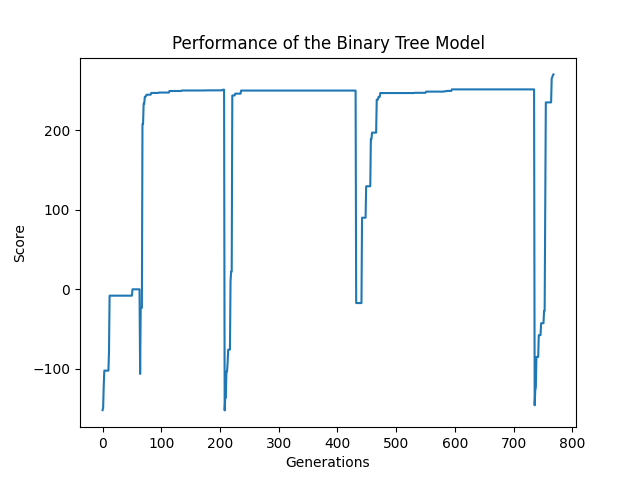
\includegraphics[width=1\linewidth]{score_generation_lineplot_lunarlander}  
       	\caption[Score over generations lineplot of the lunar lander environment]{
			\textbf{Score over generations lineplot of the lunar lander environment.} Evolutions of the best performing individual in the lunar lander environment with an increasing binary tree size over the generations.
			}
		\label{fig:lunar_lineplot}
    \end{subfigure}%
    \hspace{1em}
    \begin{subfigure}{0.48\textwidth}
        \centering
        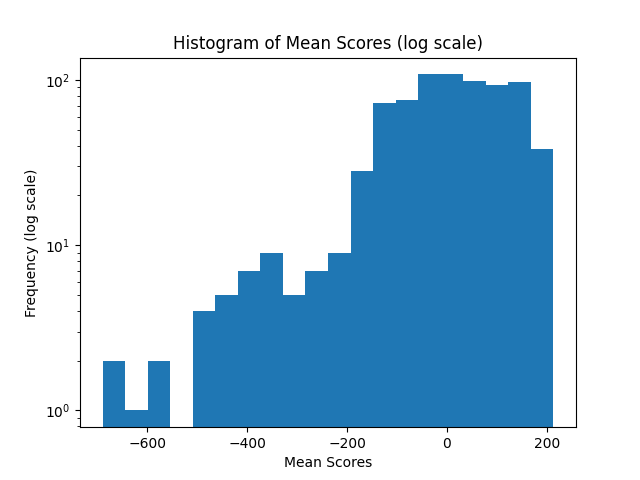
\includegraphics[width=1\linewidth]{mean_scores_histogram_lunarlander}  
        \caption[Log-scale histogram of the mean scores obtained in the lunar lander environment]{
  			\textbf{Log-scale histogram of the mean scores obtained in the lunar lander environment} The scores where obtained with a growing binary tree until one individual obtained a score of at least 270 points.
  			}
  		\label{fig:lunar_histogram}
    \end{subfigure}
    \caption{Performance plots of the lunar lander experiment.}
    \label{fig:lunar_lander_plots}
\end{figure}

\subsection{Bipedal walker}
The Bipedal Walker was not solved with the current implementation, as 300 (-300 for CMA-ES) points were not obtained throughout the experiment. However, a larger tree seemed to find more individuals with high fitness. In this experiment, the initial structure showed better results when starting with a constant as the single node's function rather than with a perceptron. The maximum number of steps was set to 1600. For the CMA-ES optimizer, the same values were chosen for the parameters as for the Lunar Lander experiment. The $stag\_step$ variable, explained in \ref{lunar_lander}, was set to 0.2 in this case.

To assess the impact of tree size on performance, the experiment was run for 45 minutes. Figure \ref{fig:bipedal_lineplot1} shows the line plot of scores over generations. Similar to the Lunar Lander, large reductions in the plot indicate an addition of nodes to the tree. With small trees, the individuals perform poorly (less than zero points). From the fifth bar onwards (which corresponds to a binary tree with nine nodes, as we start with one node and always add two nodes with the \texttt{add\_node} function), the score of the best-performing individuals with the model increases rapidly, achieving scores over 100 points. However, it is important to note that this is not always the case. Some experiments achieve lower scores even with big tree structures. For example, when the experiment was run for one hour, the results in Figure \ref{fig:bipedal_lineplot2} showed different results. The fourth and sixth bars indicate very high scores (seven and eleven nodes), but the fifth and seventh bars show that the individuals had scores of less than zero points (nine and thirteen nodes). This shows that an increasing size of the tree does not necessarily mean that individuals with high scores will be generated. In the case of this example, the highest scores were obtained with a tree structure of seven nodes.
\begin{figure}[!ht]
    \centering
    \begin{subfigure}{0.48\textwidth}
		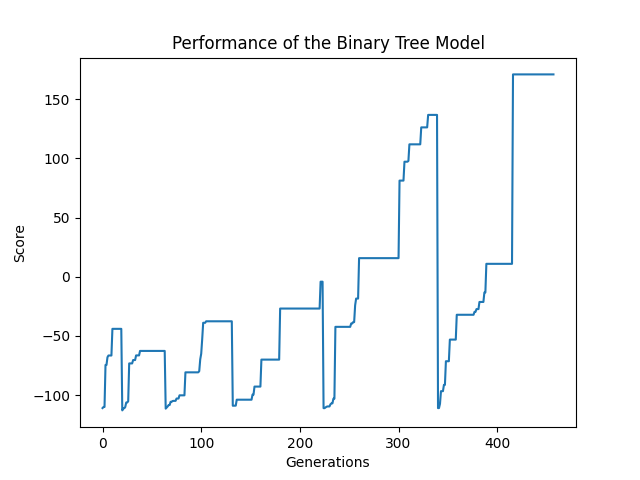
\includegraphics[width=1\textwidth]{score_generation_lineplot_bipedalwalker45}
		\caption[Lineplot of the bipedal walker environment run for 45 minutes]{
			\textbf{Score over generations lineplot of the bipedal walker.} Evolutions of the best performing individual in the bipedal walker environment run for 45 minutes with an increasing binary tree size over the generations.
			}
		\label{fig:bipedal_lineplot1}
    \end{subfigure}%
    \hspace{1em}
    \begin{subfigure}{0.48\textwidth}
        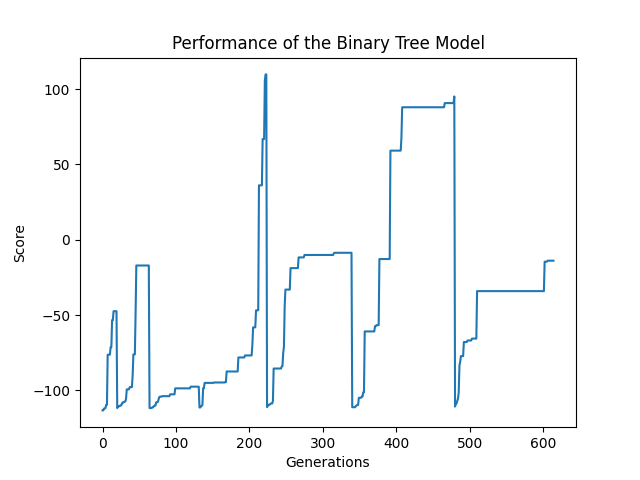
\includegraphics[width=1\textwidth]{score_generation_lineplot_bipedalwalker1h}
		\caption[Lineplot of the bipedal walker environment run for 1 hour]{
  			\textbf{Score over generations lineplot of the bipedal walker.} Evolutions of the best performing individual in the bipedal walker environment run for one hour with an increasing binary tree size over the generations.
  			}
		\label{fig:bipedal_lineplot2}
    \end{subfigure}
    \caption{Score over generations line plot of the bipedal walker environment after running the experiment for 45 minutes and 1 hour.}
    \label{Score over generations line plot of the bipedal walker}
\end{figure}

The log-scaled histogram in Figure \ref{fig:bipedal_histogram1} provides the mean scores of the populations, as calculated over 15 individuals. The experiment was run for 45 minutes. The histogram shows that, given the complexity of the environment, a large proportion of populations had low mean scores. Most of the means were below zero points and the amount decreased as the mean scores increased. There were no populations with a mean score over 20 points after 45 minutes of the experiment, which indicates that the task is still far from being solved (the target score is 300 points). The results of the same histogram after running the experiment for one hour (Figure \ref{fig:bipedal_histogram2}) showed similar results.

\begin{figure}[!ht]
    \centering
    \begin{subfigure}{0.48\textwidth}
		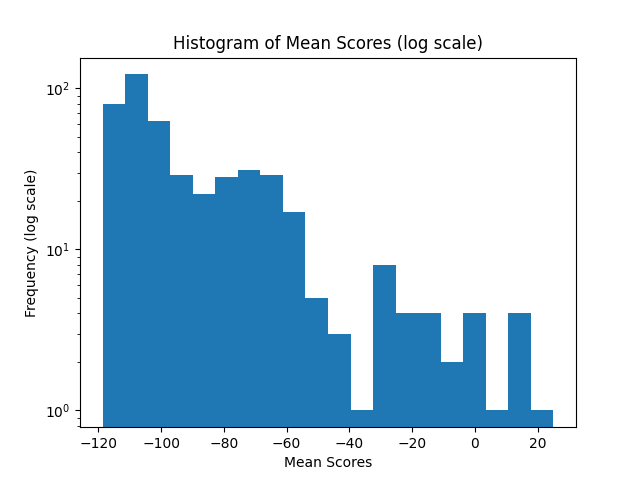
\includegraphics[width=1\textwidth]{mean_scores_histogram_bipedalwalker45}
		\caption[Log-scale histogram of the mean scores obtained in the bipedal walker environment run for 45 minutes]{
			\textbf{Log-scale histogram of the mean scores obtained in the bipedal walker environment run for 45 minutes.} The scores where obtained with a growing binary tree for one hour even if the environment was not solved.
			}
		\label{fig:bipedal_histogram1}
    \end{subfigure}%
    \hspace{1em}
    \begin{subfigure}{0.48\textwidth}
        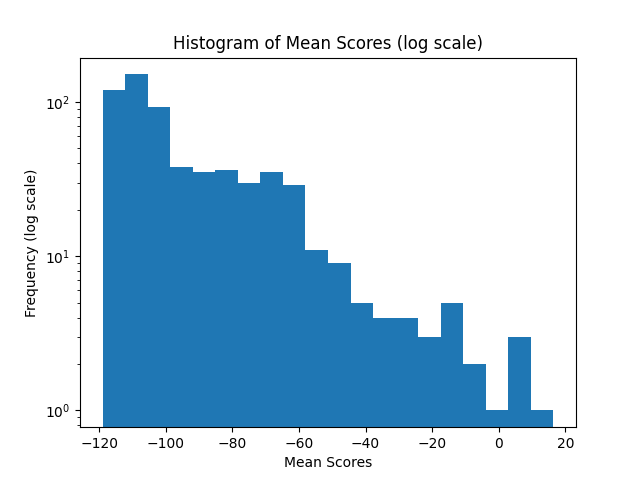
\includegraphics[width=1\textwidth]{mean_scores_histogram_bipedalwalker1h}
		\caption[log-scale histogram of the mean scores obtained in the bipedal walker environment run for 1 hour]{
  			\textbf{Log-scale histogram of the mean scores obtained in the bipedal walker environment run for 1 hour.} The scores where obtained with a growing binary tree for one hour even if the environment was not solved.
  			}
		\label{fig:bipedal_histogram2}
    \end{subfigure}
    \caption{Log-scale histogram of the mean scores obtained in the bipedal walker environment after running the experiment for 45 minutes and 1 hour.}
    \label{Log-scale histogram of the mean scores obtained in the bipedal walker}
\end{figure}

It is important to note that all of these experiments were run using the default reward functions, without fitness shaping. In the case of the more complex Bipedal Walker environment, this led to suboptimal results. The walker often became stuck in local optima, which prevented it from exploring better ways of moving. For example, the walker often remained balanced on its two legs without falling, as shown in Figure \ref{fig:bipedal_walker_local}. This is because it does not receive a large penalty for remaining in that state, whereas taking a step forward, which could lead to learning a more efficient way to walk, would result in a fall and a penalty.

\begin{figure}[!ht]
    \centering
    \begin{subfigure}{.3\textwidth}
        \centering
        \fbox{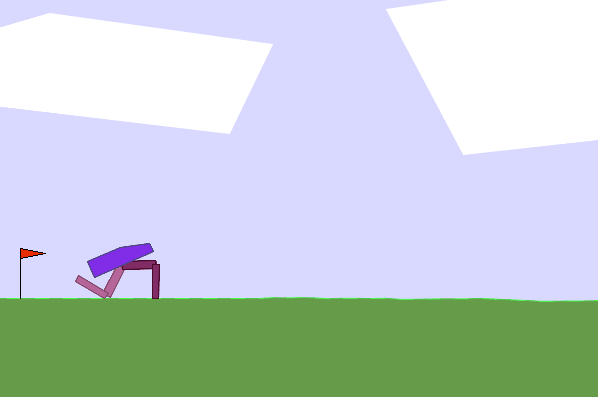
\includegraphics[width=1.05\linewidth]{bipedal_walker}}  
    \end{subfigure}
    \hspace{1em}
    \begin{subfigure}{.3\textwidth}
        \centering
        \fbox{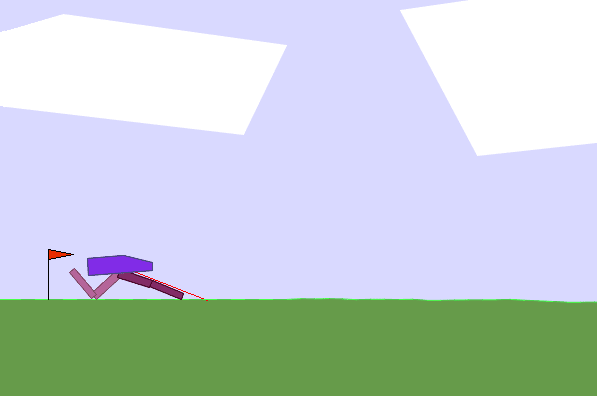
\includegraphics[width=1.05\linewidth]{bipedal_walker2}}  
    \end{subfigure}
    \hspace{1em}
    \begin{subfigure}{.3\textwidth}
        \centering
        \fbox{\includegraphics[width=1.05\linewidth]{Bipedal_walker3}}  
    \end{subfigure}
    \caption{Different states of the Bipedal walker environment where the walker got stuck in local optima.}
    \label{fig:bipedal_walker_local}
\end{figure}





 